\documentclass{beamer}
\usepackage{beamerthemesplit}
\usetheme{SPbGU}
%{CambridgeUS}
% Выпишем часть возможных стилей, некоторые из них могут содержать
% дополнительные опции
% Darmstadt, Ilmenau, CambridgeUS, default, Bergen, Madrid, AnnArbor,Pittsburg, Rochester,
% Antiles, Montpellier, Berkley, Berlin
\usepackage{pdfpages}
\usepackage{amsmath}
\usepackage{cmap} % for serchable pdf's
\usepackage[T2A]{fontenc} 
\usepackage[utf8]{inputenc}
\usepackage[english,russian]{babel}
\usepackage{indentfirst}
\usepackage{amsmath}
\usepackage{dot2texi}
\usepackage{tikz}
\usepackage{graphicx}
\usepackage{epstopdf}
\usetikzlibrary{shapes,arrows}
% Если у вас есть логотип вашей кафедры, факультета или университета, то
% его можно включить в презентацию.

%\usefoottemplate{\vbox{}}%  \tinycolouredline{structure!25}% {\color{white}\textbf{\insertshortauthor\hfill% \insertshortinstitute}}% \tinycolouredline{structure}% {\color{white}\textbf{\insertshorttitle}\hfill}% }}

%\logo{
\includegraphics[width=1cm]{SPbGU_Logo.png}}

\title[]{Генератор абстрактных лексических анализаторов}
\institute[СПбГУ]{
Санкт-Петербургский государственный университет \\
Математико-Механический факультет \\
Кафедра системного программирования }

\author[Полубелова Марина]{Полубелова Марина Игоревна \\
  \and  
  {\bfseries Научный руководитель:} магистр информационных технологий С.В. Григорьев \\ 
}

\date{22 мая 2014г.}

\begin{document}
{
\begin{frame}
    \begin{center}
        {
\includegraphics[width=1cm]{SPbGU_Logo.png}}
    \end{center}
    \titlepage
\end{frame}
}

\begin{frame}
	\transwipe[direction=90]
	\frametitle{Область применения}
	\begin{itemize}
		\item Реинжиниринг программного обеспечения
			  \begin{itemize}
                    \item Анализ и трансформация систем, код которых содержит встроенные языки
	          \end{itemize}
		\item Поддержка встроенных языков в IDE
			  \begin{itemize}
                    \item Статический поиск ошибок
	                \item Подсветка синтаксиса
	                \item Рефакторинги
	         \end{itemize}
	\end{itemize}
\end{frame}

\begin{frame}
	\transwipe[direction=90]
	\frametitle{Пример встроенного языка}
    \begin{center}
        {\includegraphics[width=0.89\linewidth]{WithoutReSharper}}
    \end{center}
\end{frame}

\begin{frame}
	\transwipe[direction=90]
	\frametitle{Пример встроенного языка}
    \begin{center}
        \onslide<1-> {\includegraphics[width=0.89\linewidth]{WithReSharper}}
        \onslide<2->{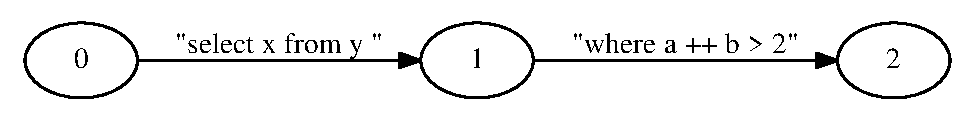
\includegraphics[width=0.89\linewidth]{Graph1}}
        \onslide<3>{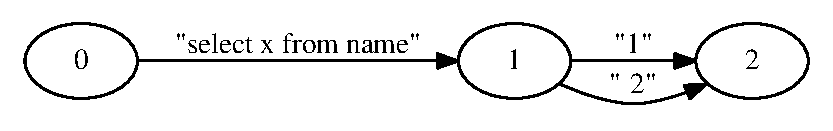
\includegraphics[width=0.89\linewidth]{Graph2}}
    \end{center}
\end{frame}

\begin{frame}[fragile]
	\transwipe[direction=90]
	\frametitle{Абстрактный лексический анализ}
	Является необходимым шагом при обработке встроенных языков. Нужен для токенизации входного графа.
	\begin{itemize}
		\item На вход анализатору подается граф, являющийся представлением динамически формируемого выражения
		\item На выходе получаем также граф, каждое ребро которого содержит токен
		\item Результирующий граф пригоден для дальнейшего синтаксического анализа
	\end{itemize}
\end{frame}


\begin{frame}
	\transwipe[direction=90]
	\frametitle{Пример}
\begin{center}
\begin{tabular}{ p{4cm} | p{5cm} }
{\centering{\textbf{\centering “Вход”}}} & {\centering{\textbf{“Лексический анализ”}}}\\
\hline
 \centering 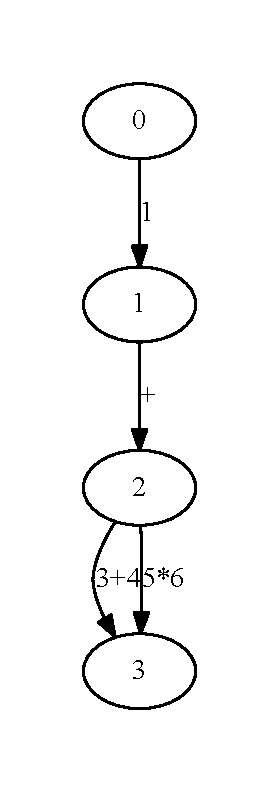
\includegraphics[height=5.5cm]{exampleGraph} & \centering 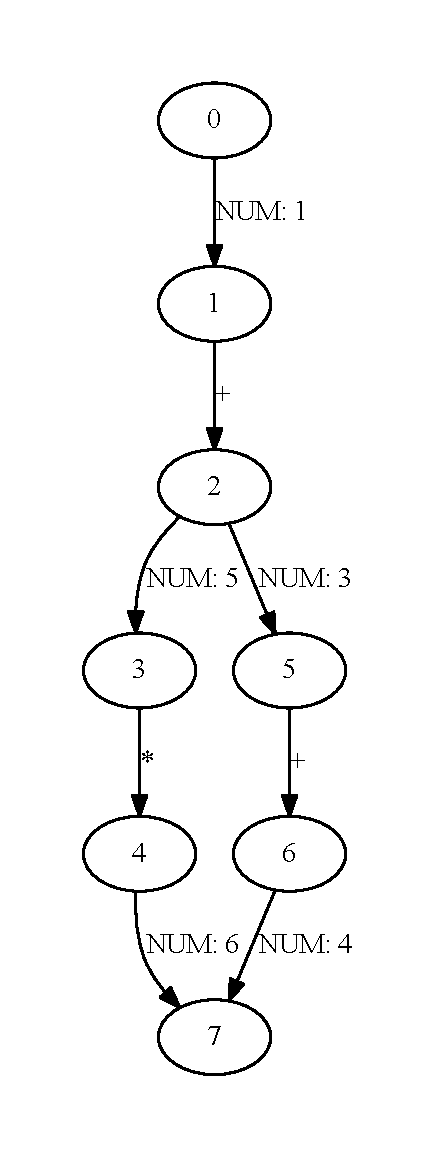
\includegraphics[height=5.5cm]{exampleGraphLexer}\\ 
\end{tabular}
\end{center}
Выражения: “1 + 3 + 4”\  и “1 + 5 * 6”
\end{frame}


\begin{frame}
	\transwipe[direction=90]
	\frametitle{Обзор существующих решений и аналогов}
	\begin{itemize}
		\item Java String Analyzer 
			\begin{itemize}
			\item строковое выражение аппроксимируют регулярной грамматикой
			\item нет лексического анализа
			\end{itemize}
		\item PHP String Analyzer
			\begin{itemize}
			\item строковое выражение аппроксимируют контексно-свободной грамматикой
			\item нет лексического анализа
			\end{itemize}
		\item Alvor
			\begin{itemize}
			\item  плагин к Eclipse для проверки встроенного в Java SQL 
			\item  проводят абстрактный лексический анализ
			\end{itemize}
		\item статья Kyung-Goo Doh, Hyunha Kim, David A. Schmidt
			\begin{itemize}
			\item  статическая валидация динамически генерируемого HTML в PHP
			\item  проводят абстрактный синтаксический анализ 
			\end{itemize}
		\item Курсовая работа Екатерины Вербицкой
	\end{itemize}
\end{frame}


\begin{frame}[fragile]
	\transwipe[direction=90]
	\frametitle{Постановка задачи}
	\begin{itemize}
	\item Доработать генератор абстрактных лексических анализаторов
		\begin{itemize}
	    	\item Поддержка “рваных”\ токенов
		    \item Сохранять привязку частей динамически формируемого выражения к исходному коду
		    \item Реализовать привязку лексических единиц внутри каждой части
	    \end{itemize}
    \item Сравнить полученный инструмент с его аналогами
    \end{itemize}
\end{frame}


\begin{frame}
	\transwipe[direction=90]
	\frametitle{Структура и принцип работы генератора}
    \begin{center}
        {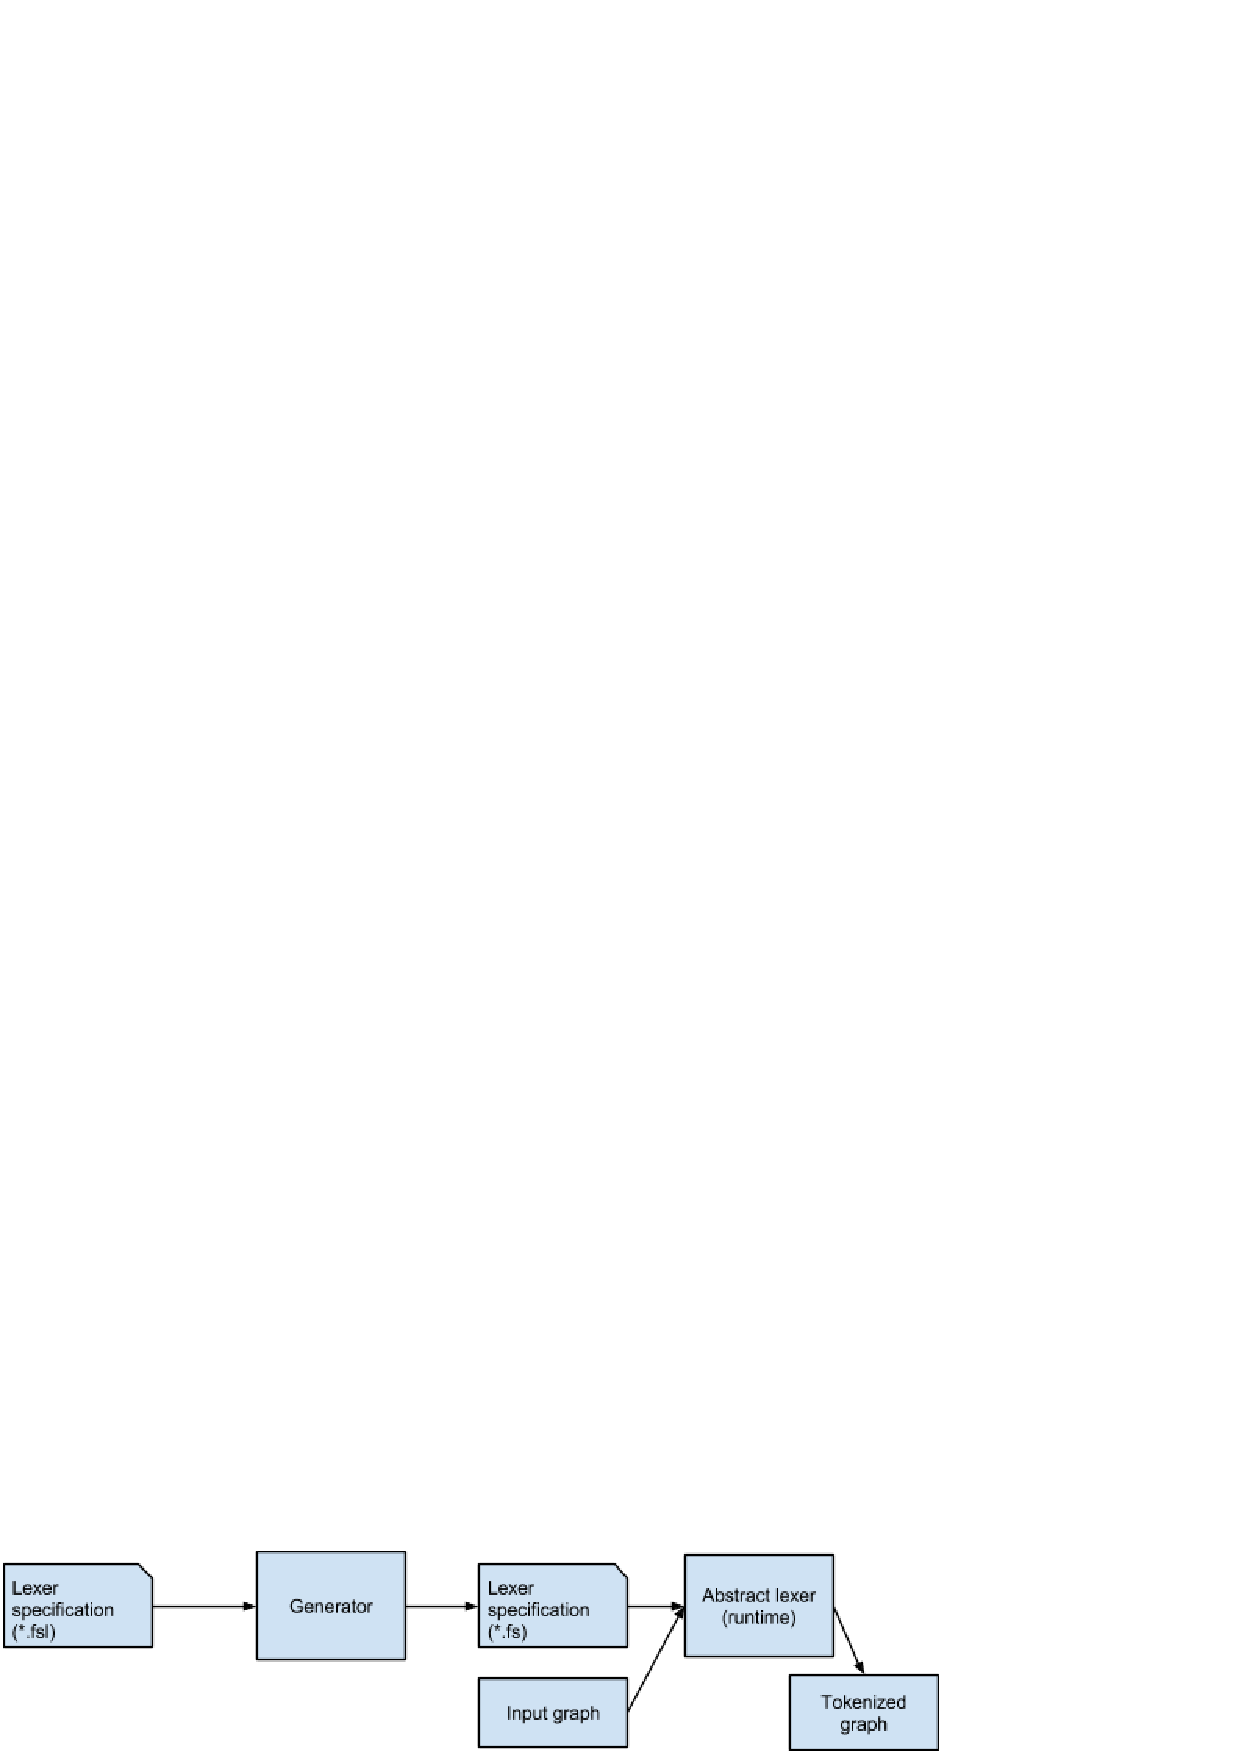
\includegraphics[width=0.9\linewidth]{Generator}}
    \end{center}
\end{frame}


\begin{frame}
	\transwipe[direction=90]
	\frametitle{Сохранение привязки к исходному коду}
	\begin{center}
	\begin{tabular}{ p{4cm} | p{5cm} }
	{\centering{\textbf{\centering “Вход”}}} & {\centering{\textbf{“Лексический анализ”}}}\\
	\hline
	\centering 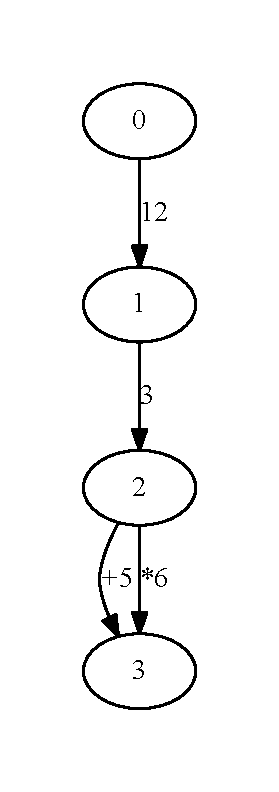
\includegraphics[height=5.5cm]{exampleBreak} & \centering 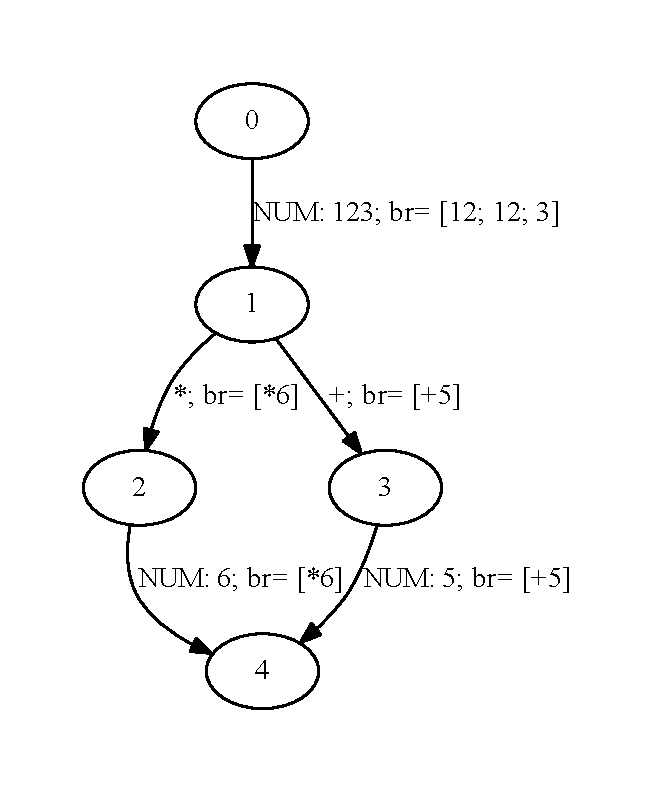
\includegraphics[height=5.5cm]{exampleBreakLexer}\
	 \end{tabular}
	 \end{center}
Выражения: “123 + 5”\  и “123 * 6”
\end{frame}

\begin{frame}
	\transwipe[direction=90]
	\frametitle{Пример работы}
    \begin{center}
		\includegraphics[width=0.89\linewidth]{WithReSharper}
    \end{center}
\end{frame}

\begin{frame}
	\transwipe[direction=90]
	\frametitle{Генерация тестов}
	Набор тестов параметризуется кратностью ребра (m = 2) и длиной цепочкой (n = 3)
	\begin{center}
	\centering 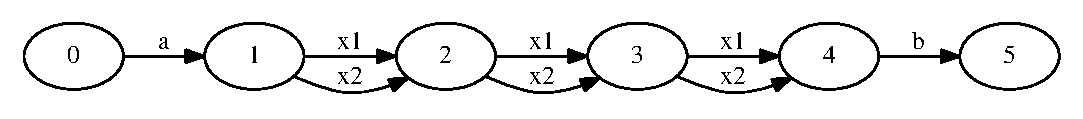
\includegraphics[width=0.89\linewidth]{m2_n3}
	 \end{center}
\end{frame}

\begin{frame}
	\transwipe[direction=90]
	\frametitle{Сравнение производительности}
	\begin{center}
	\centering 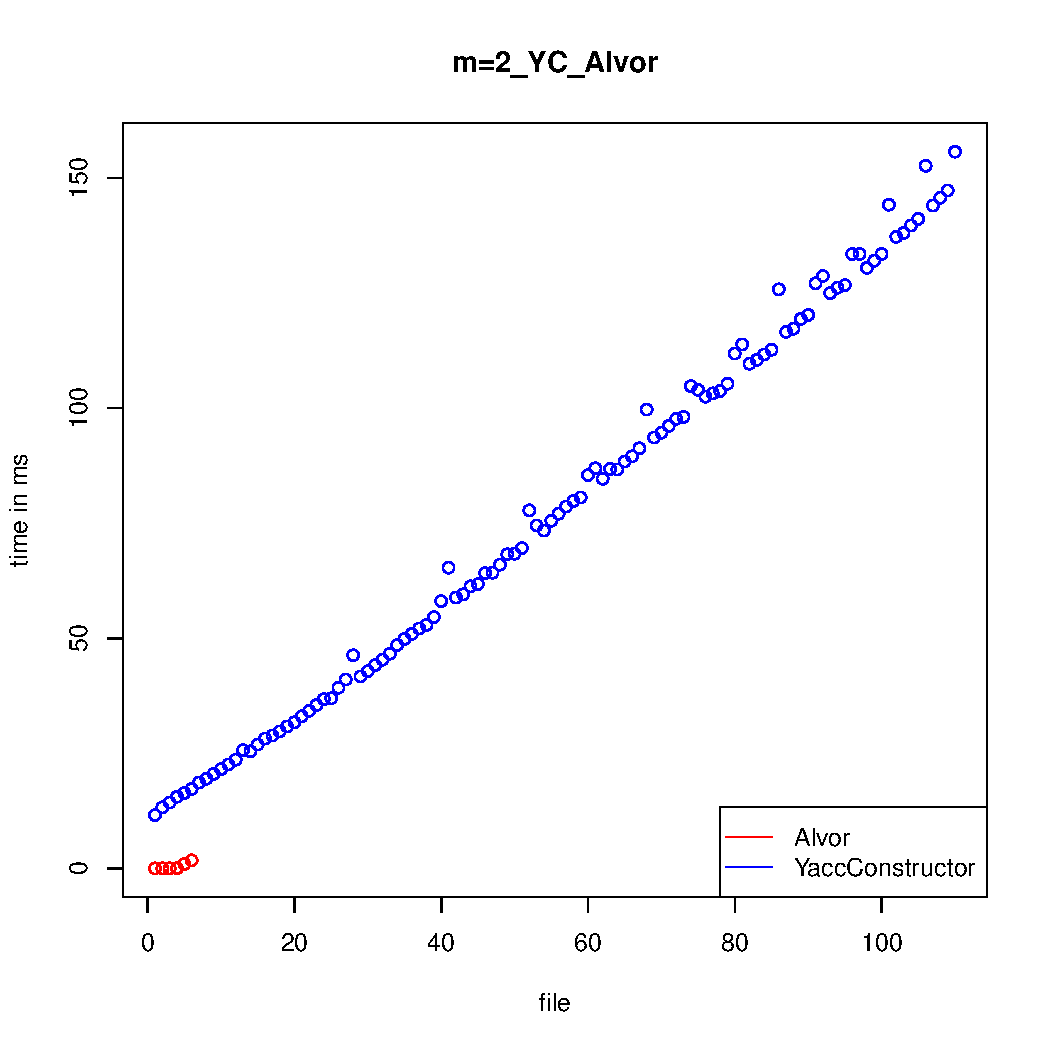
\includegraphics[width=0.65\linewidth]{m=2_YC_Alvor}
	 \end{center}
\end{frame}

\begin{frame}%[t]
	\transwipe[direction=90]
	\frametitle{Результаты}
	\begin{itemize}
		\item Реализована структура, хранящая информацию о позиции токена в исходном коде
        \item Осуществлена корректная передача координат токена к ReSharper
        \item Изучены аналоги лексических анализаторов
		\item Реализован инструмент для тестирования лексеров YaccConstructor и Alvor
        \item Проведено сравнение лексера инструментов YaccConstructor и Alvor на одинаковых входных данных
        \item Результаты работы представлены на конференции “Технологии Microsoft в теории и практике программирования”
        \item Принята статья “Инструментальная поддержка встроенных языков в интегрированных средах разрботки” на семинар по наукоёмкому ПО.
	\end{itemize}
\end{frame}

\end{document}
